\documentclass[a4paper, 12pt, notitlepage]{article}
\usepackage[margin=0.5in]{geometry}
\usepackage[utf8x]{inputenc}
\usepackage{fancyhdr}
\usepackage{amsmath}
\usepackage{amssymb}
\usepackage{gensymb}
\usepackage[makeroom]{cancel}
\usepackage{tikz}
\usepackage{float}
\usepackage[final]{pdfpages}
\usepackage{graphicx}
\usepackage{tabularx}
\usepackage{hyperref}

\title{Computational Biology - 3$^\text{rd}$ Assignment}
\author{Nicolás Espinoza Muñoz}
\date{November 20, 2020}

\newcommand\numberthis{\addtocounter{equation}{1}\tag{\theequation}}
\pagenumbering{gobble}

\begin{document}
\maketitle
\subsubsection*{Introduction}
When it comes to drug design, computational methods are becoming more important as time passes. The Quantitative Structure-Activity Relationship analysis, or QSAR, has been at the front in the field, since it proves to be both of easy implementation and very powerful. It offers a quantification of the influence of a particular bioactive molecule or family of molecules on the biological activity of the target system, usually a cell. In the following we will answer the questions presented as part of the third assignment of the Computational Biology course, which focuses on the 2D QSAR methods of Free-Wilson and Hansch analysis, as well as a 3D QSAR study of electrostatic and steric effects.

\section*{Questions}
We will directly include the questions of the assignment into this report, and in the next section proceed to answer them, as it's simpler this way.
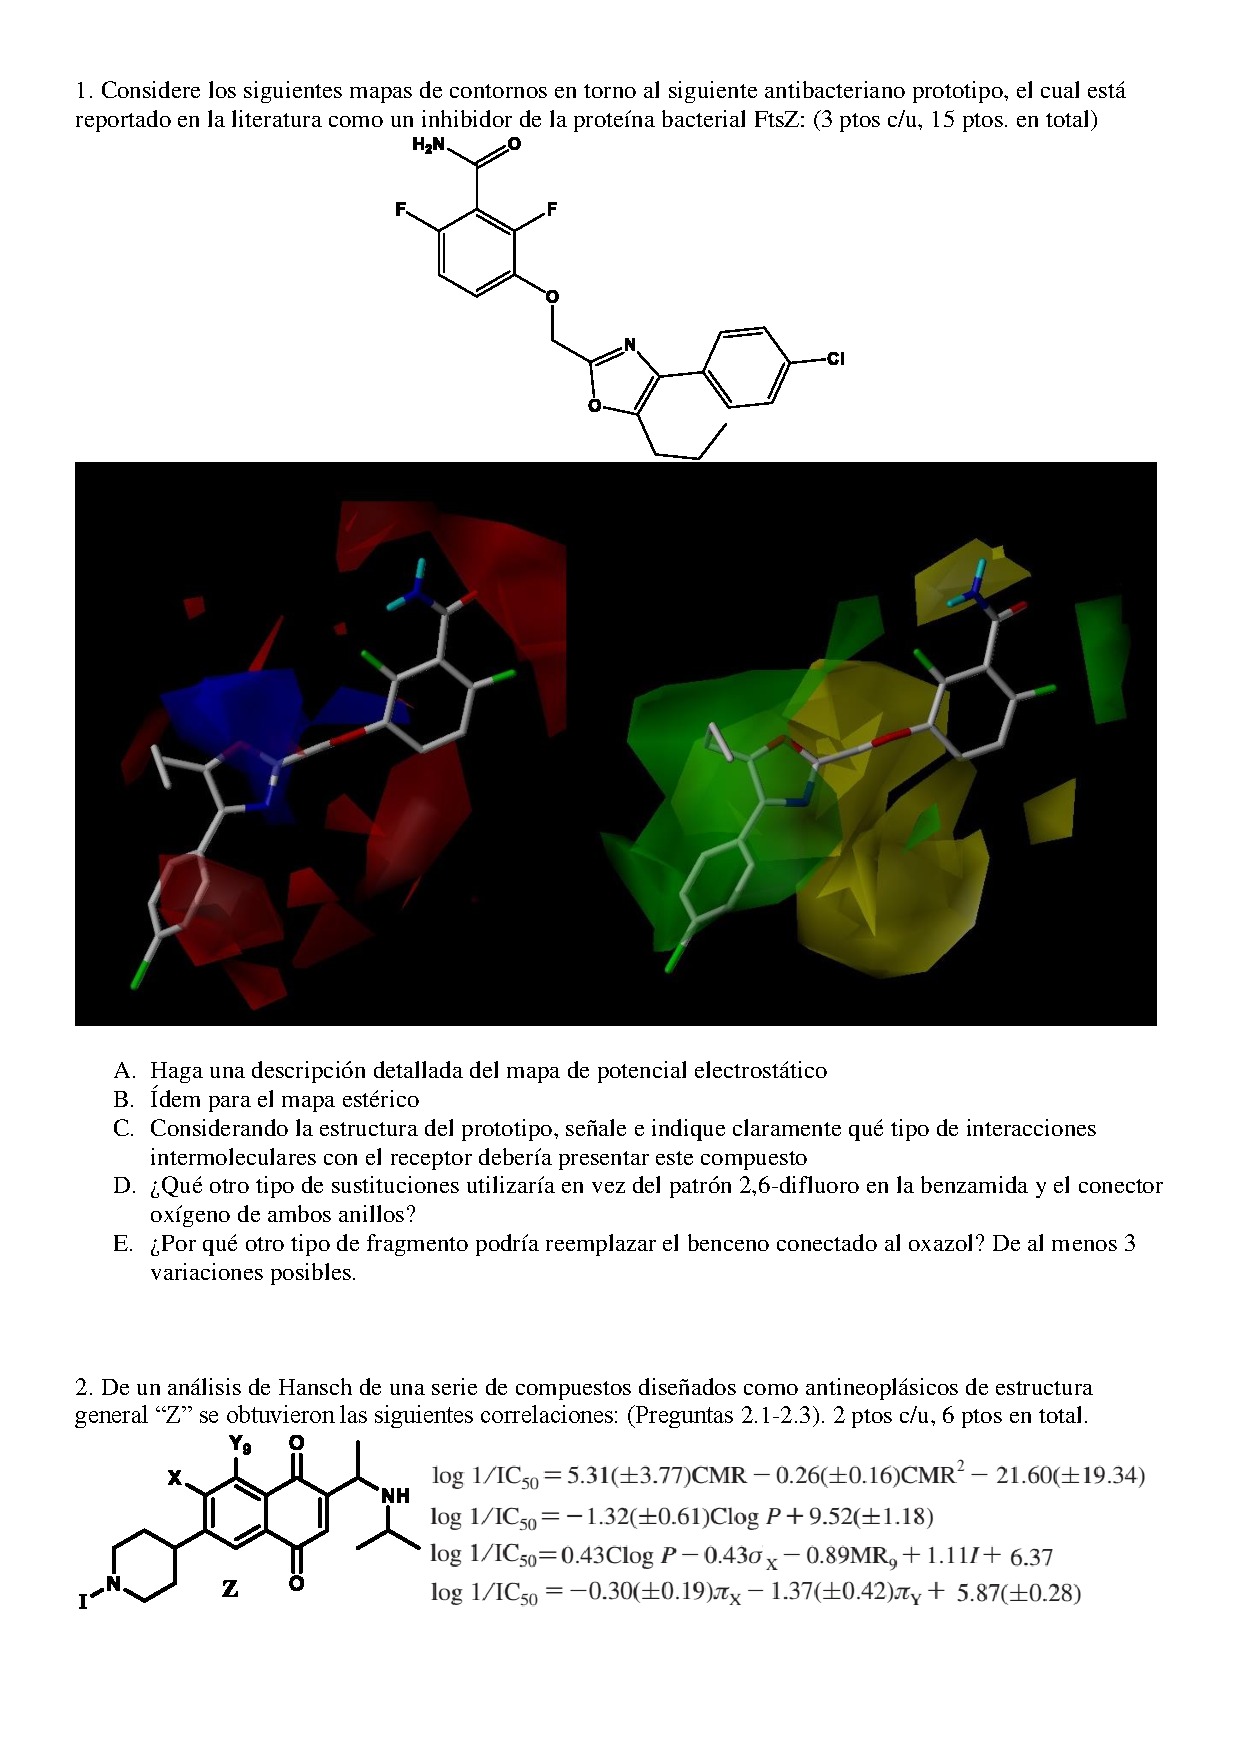
\includepdf[pages=-]{Tarea3_enunciado.pdf}

\section*{Answers}
\subsection*{1.}
\subsubsection*{A}
The electrostatic potential reveals which sections of the molecule would benefit from the insertion of electron rich (red) or electron deficient (blue) atoms or groups. The carboxamido substituent from the benzamide is not sufficiently rich in electrons; the same appears to happen with one of the fluorine atoms, and therefore the potential map relative to them shows in red. Likewise, the electrostatic potential corresponding to the lower spatial portion of both six-membered benzene rings is also red, which reveals that currently those components of the molecule are electron deficient and should be replaced by electron-rich groups. The ring-connecting oxygen seems electron rich, as does the majority of the oxazole ring, because the spatial representation of the potential around those components is blue. The smaller polyhedrons are to be ignored, as they are representative of lesser electrostatic effects.
\subsubsection*{B}
The steric map represents the volumetric information of the current molecule; green sections mean a bigger substituent, in terms of volume, is more beneficial. Conversely, yellow polyhedra correspond to groups or elements that have too big a volume. In the map presented, the oxazole and the benzene ring directly connected to it appear to be too small, and it is better to include bigger groups. Surrounding the oxygen that connects the oxazole to the benzamide, as well as part of the benzene ring of the benzamide, is a massive yellow polyhedron. This shows it is convenient to replace some elements in that section with smaller groups. It also looks like the volume of the NH$_\text{2}$ in the amide group is a bit too large, and one of the fluorine atoms connected to the benzamide could be replaced with something with a bigger volume.\footnote{Bigger and smaller are used to refer to volume.}
\subsubsection*{C}
-
\subsubsection*{D}
Based on the steric map, we should replace fluoride atoms by something with a bigger volume, but not too much, so an answer would be a chlorine in each position. As for the ring connector, a carbon is the only thing that comes to mind, because we have to replace the oxygen with an element with less electrons and less volume.
\subsubsection*{E}
-
\subsection*{2}
Only the explanations as to why a statement is considered true or false, together with the letter of the chosen alternative, are presented next. The statement itself is not quoted.
\subsubsection*{2.1}
\begin{itemize}
	\item[I.] False: From the correlations of the Hansch analysis, $\pi_X$ and $\pi_Y$ have a negative factor, so a higher lipophilicity would lower the Biological Activity. This also happens for the second correlation with $C\log P$. The only exception would be $C\log P$ in the third correlation. Then again, when lipophilicity is too high, the molecule will likely just remain in the membrane and no actually enter the cell.
	\item[II.] False: For high values of CMR, the term CMR$^2$ will be more important to Biological Activity, simply because it scales with the square of CMR.
	\item[III.] False: The presence or absence of an ethyl group affects the third correlation, but that is a Free-Wilson of term, and not lipophilicity.
	\item[IV.] True: The lower the lipophilicity of X and Y, the better, because they are factored by a negative term.
\end{itemize}
\textbf{Answer}: a) solo IV

\subsubsection*{2.2}
\begin{itemize}
	\item[I.] True: A lower lipophilicity and electron donor group is better for the Biological Activity. $\sigma_X$ and $\pi_X$ are factored by negative terms, so a lower $\pi_X$ and $\sigma_X$ are both beneficial for these correlations.
	\item[II.] False: As chlorine is smaller in terms of volume, its lipophilicity is lower, and since $\pi_Y$ is factored by a negative term, that's the better scenario.
	\item[III.] False: NO$_\text{2}$ and CN groups are electron deficient, so they have a positive Hammett's sigma value. Since the factor multiplying $\sigma_X$ is negative, this would not be a beneficial substituent.
	\item[IV.] False: We have to check the factors of the $\sigma$, $\pi$ and $\log P$ terms. Those multiplying $\pi_{X}$, $\pi_Y$ and $\log P$ are bigger than that multiplying $\sigma_X$.
\end{itemize}
\textbf{Answer}: a) solo I

\subsubsection*{2.3}
\begin{itemize}
	\item[I.] We can know this; we have correlations with both $\sigma_X$ and $\pi_X$. It is false though.
	\item[II.] We can't know this; we have no $\sigma_Y$ term in any of the correlations presented.
	\item[III.] We can't know this; there is no information regarding the molar refractivity (MR) of \textit{I}.
	\item[IV.] We can know this; we have the corresponding term in at least one of the correlations.
\end{itemize}
\textbf{Answer}: a) II y III

\subsection*{3}
For this exercise we added two columns, one per table, as there were columns with values that rose way past 1. So for the first table, we added a $\pi_X^2$ column, and for the second we added a MR$_Y^2$ column. We now present both equations, (1) for Table 1 of the exercise, and (2) for Table 2. These were obtained with Multiple Linear Regression. For Table 1 we used 10 out of the 14 lines of information available, and for Table 2 we used 12 out of 17. This accounts for roughly 70\% of the data available in each case. We then used the remaining data to verify the correlations obtained.
\begin{equation}
	\log\left(\frac{1}{EC_{50}}\right) = -0.398(\pm 0.398)\pi_X + 0.020(\pm 0.178)\pi_X^2 - 1.385(\pm 0.258)\pi_Y + 5.927(\pm 0.203)
\end{equation}
\begin{gather*}
	\log\left(\frac{1}{EC_{50}}\right) = 1.057(\pm 0.502)\text{MR}_Y - 0.749(\pm 0.258)\text{MR}_Y^2 + 0.797(\pm 0.249)I \\ + 0.253(\pm 0.188)I_1 + 6.406(\pm 0.184) \numberthis
\end{gather*}
Before continuing with the answers requested, the point has to be made that the second correlation actually fails to return a good value of $\log p$ for some data in the Table 2 set. We tried many different variable combinations between MR$_Y$, MR$_Y^2$, $I$ and $I_1$, sometimes excluding one or more of those terms, but failed to get results that were substantially better, so the decision was made to present correlation (2) as is.
\subsubsection*{a)}
It is convenient, at least basing the answer in the median factor obtained for each $\pi$, that $\pi_X$ and $\pi_Y$ both be small. Given the correlation (1), it is better to have hydrophilicity rather than lipophilicity.
\subsubsection*{b)}
Molar refractivity should be higher than $1$ but not too much, because there is a point where the MR$_Y^2$ term, which has a negative factor, begins to dominate. This means there is a limit to how much a bigger volume is beneficial in terms of the $\log(1/EC_{50})$ indicator.
\subsubsection*{c)}
It is convenient that there be a methyl group in the X group position, as shown by the positive factor accompanying $I_1$.
\subsubsection*{d)}
According to our correlations, it is indeed good for the molecule to have an imide group in the Y position; the reason is the same as for letter c).
\subsubsection*{e)}
For compound number 1, the main property is lipophilicity of the group occupying position Y. For compound number 2, the main factor would be the molar refractivity of the substituent that should go in position Y as well, although one could make the point that it is also important to consider the presence of imide in Y, as it has the second highest factor in the correlation.
\subsubsection*{f)}
-

\section*{Conclusions}
QSAR methods are a powerful tool to design bioactive molecules, as they allow us to develop and test molecules directly on the computer, before going onto live tests. It is also rather simple to formulate these correlations, and a researcher has a lot of flexibility when it comes to component replacements for testing different drugs, given there is data about the parameters of special interest for each case. The catch is, one has to be rather knowledgeable about the compatibility of each substituent being considered as part of the compound family studied, and has to be able to correctly interpret the correlations obtained. Also, this field actually integrates a good amount of disciplines, from statistics to electrostatics, and of course chemistry, so it is by no means a simple subject.\\\\
Here we tried to show, at least partially, how useful the QSAR techniques are for identifying relevant properties in the Biological Activity influence a specific molecule has, and went on to produce and interpret our own correlations. We also studied 3D QSAR methods, which allow us to study non-planar models of molecules, so one could argue they are in fact more precise in some ways. Nevertheless, 2D and 3D QSAR methods remain important as they immensely facilitate bioactive molecule design and reduce the costs associated with it.
\end{document}